\documentclass{article}
%---------------packages--------------------
\usepackage[utf8]{inputenc}
\usepackage{tikz}
\usepackage{comment}
\usetikzlibrary{calc}
%---------------title-----------------------
\title{Drawing}
\author{Yasin Hassan}
\date{\today}

%---------------document--------------------
\begin{document}
\maketitle
\begin{figure}[h] %h towards top of document
\centering
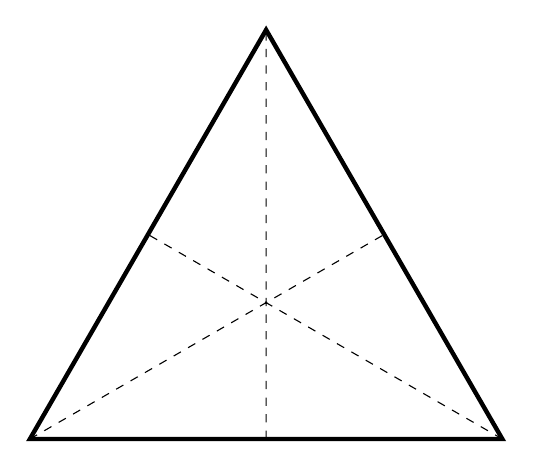
\begin{tikzpicture}[scale = 3] %there's also scale and yscale
%\draw (0,0)--(2,0)--(1,1.73205)--(0,0); 
%cycles to starting point, can also write {0,0)all lengths in centimeters
\draw[ultra thick] (0,0)--(2,0)--(1,{sqrt(3)})--cycle; %why not \sqrt?
\draw[dashed] (1,0)--(1,{sqrt(3)}) (0,0)--(1.5, 0.866) (2,0) -- (0.5, 0.866);
\end{tikzpicture}
\caption{My triangle}
\end{figure}

\begin{figure}[h]
\centering
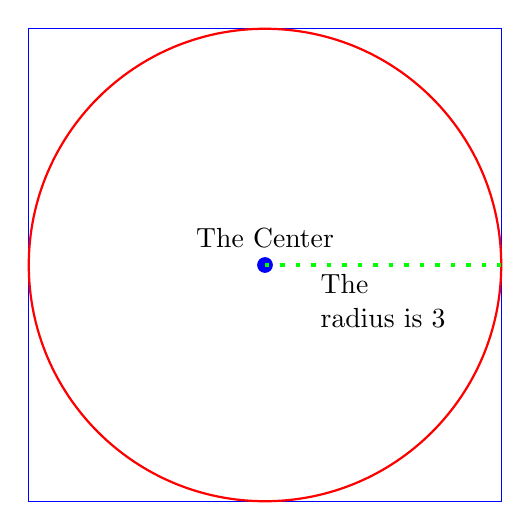
\begin{tikzpicture}
\draw[blue] (-3,-3) rectangle (3,3);
\draw[red, thick] (0,0) circle [radius = 3];
%\draw[fill, blue] (0,0) circle [radius = 0.1];%both fill circles work
\fill[blue] (0,0) circle [radius = 0.1];
\draw[green, loosely dotted, ultra thick] (0,0)--(3,0);
\node[above] at (0,0.1) {The Center};%above below left right
\node [below, align = left] at (1.5,0) {The\\ radius is 3};
\end{tikzpicture}
\end{figure}

\begin{figure}[h]
\centering
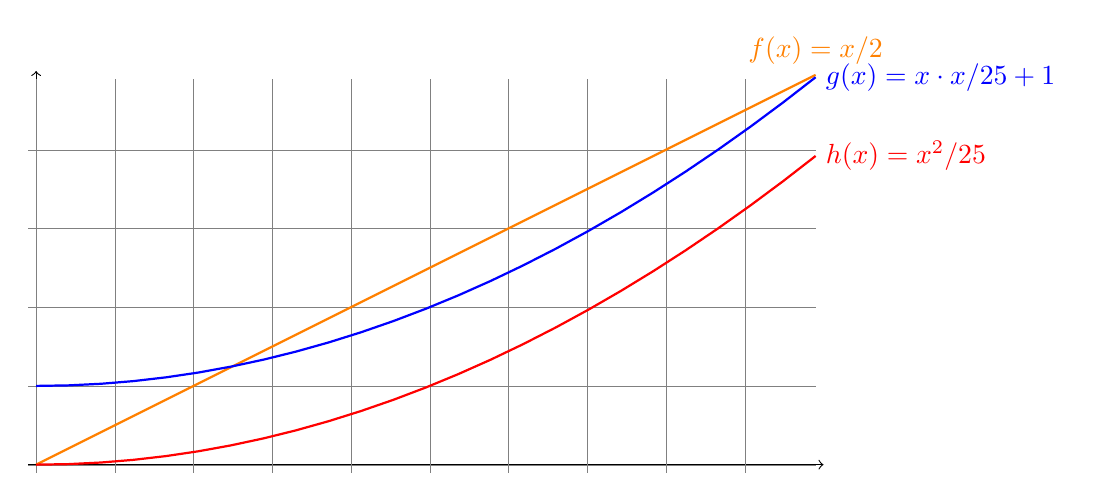
\begin{tikzpicture}[domain = 0:9.9]
\draw[->] (-0.1,0) -- (10,0);
\draw[->] (0,-0.1) -- (0,5);
\draw[gray, ultra thin] (-0.1,-0.1) grid (9.9,4.9);
\draw[orange, thick] plot (\x, \x/2) node[above]{$f(x)=x/2$};
\draw[blue, thick] plot(\x,\x*\x/25+1) node[right]{$g(x)=x\cdot x/25 + 1$};
\draw[red,thick] plot(\x,{pow(\x,2)/25}) node[right]{$h(x)=x^2/25$}; %always place functions with multiple parentheses in {}
\end{tikzpicture}
\end{figure}

\begin{figure}[h]
\centering
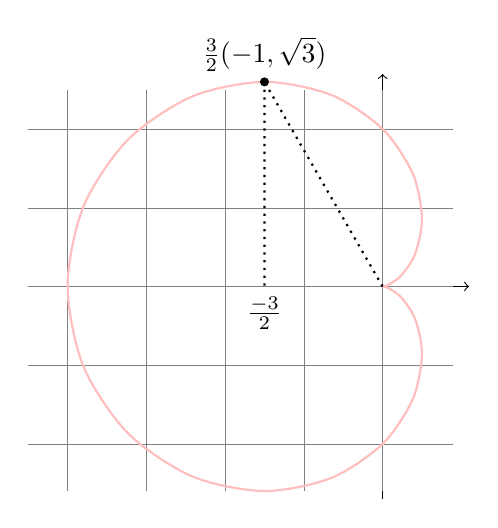
\begin{tikzpicture}[domain = 0: 2*pi]
\draw[->] (0,-2.7) -- (0,2.7);
\draw[->] (-4.5,0) -- (1.1,0);
\draw[gray, ultra thin] (-4.5,-2.6) grid (0.9,2.5);
\draw[smooth, pink, thick] plot ({2*(1-cos(\x r))*cos(\x r)},{2*(1-cos(\x r))*sin(\x r)}); % r radians
%2pi/3
\draw[dotted, thick] (0,0)--({2*(1-cos(2*pi/3 r))*cos(2*pi/3 r)},{2*(1-cos(2*pi/3 r))*sin(2*pi/3 r)}) node[above]{$\frac{3}{2}(-1,\sqrt{3})$};
\draw[fill] ({2*(1-cos(2*pi/3 r))*cos(2*pi/3 r)},{2*(1-cos(2*pi/3 r))*sin(2*pi/3 r)}) circle [radius = 0.05];
\draw[dotted, thick] ({2*(1-cos(2*pi/3 r))*cos(2*pi/3 r)},{2*(1-cos(2*pi/3 r))*sin(2*pi/3 r)}) -- (-3/2,0) node[below]{$\frac{-3}{2}$};
\end{tikzpicture}
\end{figure}

\begin{figure}[h]
\centering
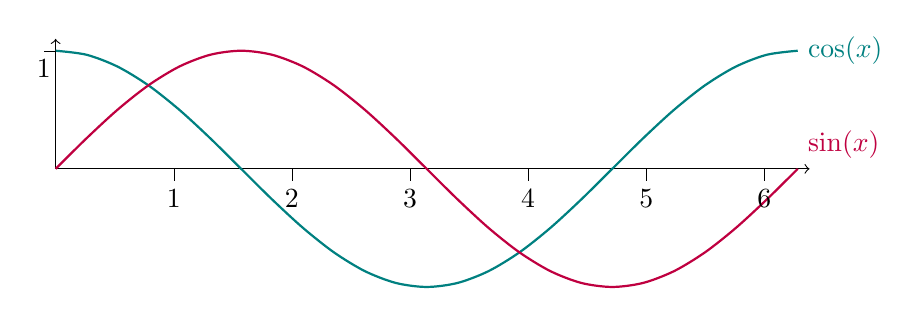
\begin{tikzpicture}[domain = 0:2*pi, scale = 1.5]
\draw[<->](2*pi+0.1,0)--(0,0)--(0,1.1);
\draw[smooth, teal, thick] plot (\x,{cos(\x r)}) node[right] {$\cos(x)$};
\draw[smooth, purple, thick] plot (\x,{sin(\x r)}) node[above right] {$\sin(x)$};
\foreach \x in {1,...,6}{
\draw[ultra thin] (\x,0)--(\x,-0.1) node[below]{$\x$};
}
\draw[ultra thin] (0,1)--(-0.1,1) node[below]{$1$};
\end{tikzpicture}
\end{figure}

\begin{figure}[h]
\centering
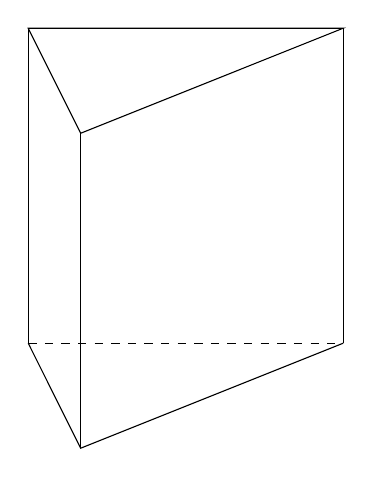
\begin{tikzpicture}
\coordinate (A) at ($2*(-1,0,0)$);
\coordinate (B) at ($2*(1,0,0)$);
\coordinate (C) at ($2*(0,0,{sqrt(3)})$);
\coordinate (H) at ($2*(0,2,0)$);
\draw (B)--(C)--(A);
\draw[dashed] (A)--(B);
\draw ($(A)+(H)$)--($(B)+(H)$)--($(C)+(H)$)--cycle;
\draw (A) --+ (H);
\draw (B) --+ (H);
\draw (C) --+ (H);
\end{tikzpicture}
\end{figure}
\end{document}